\documentclass[11pt]{article}
\usepackage[paperwidth=254mm,paperheight=142.875mm,margin=12mm]{geometry}
\usepackage{amsmath,amssymb}
\usepackage{graphicx}

\newcommand{\R}{\mathbb{R}}

\newcommand{\slide}[1]{\clearpage\noindent{\Large\bfseries #1}\par\vspace{4pt}\hrule\vspace{10pt}}

\begin{document}

% TITLE SLIDE
\clearpage
\vspace*{\fill}
\begin{center}
{\LARGE\bfseries Robust Training of Neural Networks\\[4pt] at Arbitrary Precision and Sparsity}\par\vspace{8pt}
{\large C.~Ye, G.~Chu, Y.~Liu, Y.~Zhang, L.~Lew, L.~Zhang, M.~Sandler, A.~Howard}\par
{\large Google DeepMind \quad\textbullet\quad ICLR 2026}\par\vspace{28pt}
{\large Presented by}\par\vspace{6pt}
{\Large Ayush Srivastava (2026AIB2015)\qquad Sarvesh Nikas (2026AIB2045)}
\end{center}
\vspace*{\fill}

\slide{Why quantization, and the forward pass during training}

\paragraph{Why quantization.} Modern neural networks are huge: a language model has billions of weights, each stored as a 32-bit or 16-bit floating-point number. This makes models too big to fit on a phone, slower to run, and costly in energy. Quantization stores each weight with far fewer bits: 4, 2 or 1 bit instead of 16 or 32.

\paragraph{Training with quantization.} During training the network keeps the float weights $x$ and updates them by gradient descent. We could compute with $x$, but we deliberately use the quantized version $\hat x$ in the forward pass, so the network learns to be robust to the rounding it will face at inference. After training, $x$ is discarded; only the low-bit integers $q$ (plus one $s_f$, $b_f$ per block) are kept.

\paragraph{The forward pass during training.}
\[
x\ \xrightarrow{\ f\ }\ f(x)\ \xrightarrow{\ \operatorname{round}\ }\ q\ \xrightarrow{\ s_f q+b_f\mathbf 1\ }\ \hat x\ \longrightarrow\ \text{rest of network}\ \longrightarrow\ L
\]
\begin{itemize}
\item $x\in\R^N$: float block, kept and updated during training.
\item $f(x)=\dfrac{x-b_f\mathbf 1}{s_f}$: rescales $x$ onto the $k$-bit integer grid; $s_f$ = grid step in real units, $b_f$ = real value of integer $0$ ($b_f=0$ in the linear case).
\item $q=\operatorname{round}\big(f(x)\big)=f(x)+\delta$: the integers, with rounding error $|\delta_i|\le\frac12$.
\item $\hat x=s_f\,q+b_f\mathbf 1=x+s_f\,\delta$: $x$ as seen after quantization; this is what the next layer uses.
\end{itemize}

\slide{The problem: the true gradient is zero}

\paragraph{Chain rule through the quantizer.} Gradient descent needs $\nabla_x L$:
\[
\nabla_x L=\Big(\frac{\partial \hat x}{\partial x}\Big)^{\!\top}\nabla_{\hat x}L,
\qquad
\frac{\partial \hat x}{\partial x}
=\underbrace{s_f}_{\text{scale back}}\cdot\underbrace{\frac{\partial q}{\partial f(x)}}_{\text{round}}\cdot\underbrace{\frac{1}{s_f}}_{f}
=\frac{\partial q}{\partial f(x)} .
\]
The two scalings cancel: the local gradient is exactly the slope of $\operatorname{round}$.

\paragraph{Round is a staircase.}
\[
\frac{d}{du}\operatorname{round}(u)=0\quad\text{for } u\notin\mathbb Z+\tfrac12,\qquad\text{undefined at } u\in\mathbb Z+\tfrac12 .
\]
Hence $\dfrac{\partial q}{\partial f(x)}=0$ almost everywhere, so
\[
\nabla_x L=0 .
\]

\paragraph{Consequence.} A small change in $x$ does not change $q$, so the loss gives $x$ no direction to move: $x$ and every layer before it never update. Training cannot start.

\slide{The standard fix: Straight-Through Estimator (STE)}

\paragraph{Idea.} Forward pass: round exactly as before. Backward pass: pass the gradient straight through the rounding, i.e.\ replace the true slope of $\operatorname{round}$ (zero) by $1$. This is a chosen rule, not a derived derivative.

\paragraph{Decomposition.} Write the rounded value as the smooth part plus the rounding error:
\[
q=\operatorname{round}\big(f(x)\big)=f(x)+\delta,
\qquad
\delta=\operatorname{stopgrad}\Big(\operatorname{round}\big(f(x)\big)-f(x)\Big),
\]
where $\operatorname{stopgrad}$ means: same value in the forward pass, treated as a constant (zero derivative) in the backward pass.

\paragraph{Forward.} $f(x)+\delta=\operatorname{round}\big(f(x)\big)$ exactly, so the network still sees quantized values.

\paragraph{Backward.} $\delta$ is a constant, so
\[
\frac{\partial q}{\partial f(x)}=\frac{\partial f(x)}{\partial f(x)}+\underbrace{\frac{\partial \delta}{\partial f(x)}}_{=\,0}=I .
\]
Substituting into the chain rule of the previous slide,
\[
\frac{\partial \hat x}{\partial x}=s_f\cdot I\cdot\frac{1}{s_f}=I,
\qquad\text{hence}\qquad
\nabla_x L=\nabla_{\hat x}L .
\]

\paragraph{Effect.} The gradient reaching $x$ is no longer zero, so $x$ and earlier layers update and training works.

\vfill
\noindent{\small\textit{Reference:} Y.~Bengio, N.~L\'eonard, A.~Courville, ``Estimating or propagating gradients through stochastic neurons for conditional computation,'' arXiv:1308.3432, 2013.}

\slide{Why STE fails: the blind spot}

\paragraph{Forward and backward disagree.}
\[
\text{forward: }\ \hat x=x+s_f\,\delta,
\qquad\qquad
\text{backward: }\ \frac{\partial \hat x}{\partial x}=I .
\]
\begin{itemize}
\item The forward pass uses the rounded values: every entry is shifted by its rounding error $s_f\delta_i$, which changes the output and the loss.
\item The local Jacobian is $I$: exactly what it would be with no quantization at all ($\hat x=x$). $\delta$ does not appear in it.
\item So earlier layers get no signal about how rounding hurts the loss, and cannot learn to be robust to it. The paper calls $\delta$ a ``ghost of departed quantities'' (Berkeley, 1754).
\item At 8 bits $s_f\delta$ is tiny and ignoring it is harmless. At 1--2 bits it is as large as the values themselves: the gradient no longer matches what the forward pass did, and training becomes unstable (STE diverges at A1W1, next slide, left).
\item With affine quantization, STE barely learns the offset: no gain over linear (next slide, right).
\end{itemize}

\slide{STE at 1 bit: results from the paper}

\noindent
\begin{minipage}[t]{0.49\textwidth}\centering
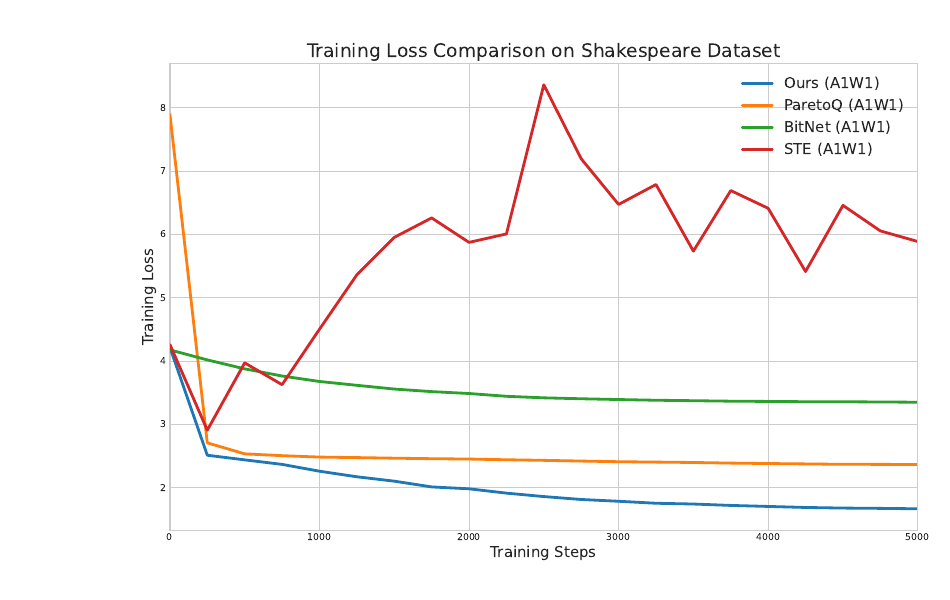
\includegraphics[width=\linewidth]{figs/fig1a_ste_divergence.png}\\[4pt]
\small Training loss, 1-bit weights and activations (A1W1), small GPT on Shakespeare. STE (red) diverges; the paper's method (blue) converges.
\end{minipage}\hfill
\begin{minipage}[t]{0.49\textwidth}\centering
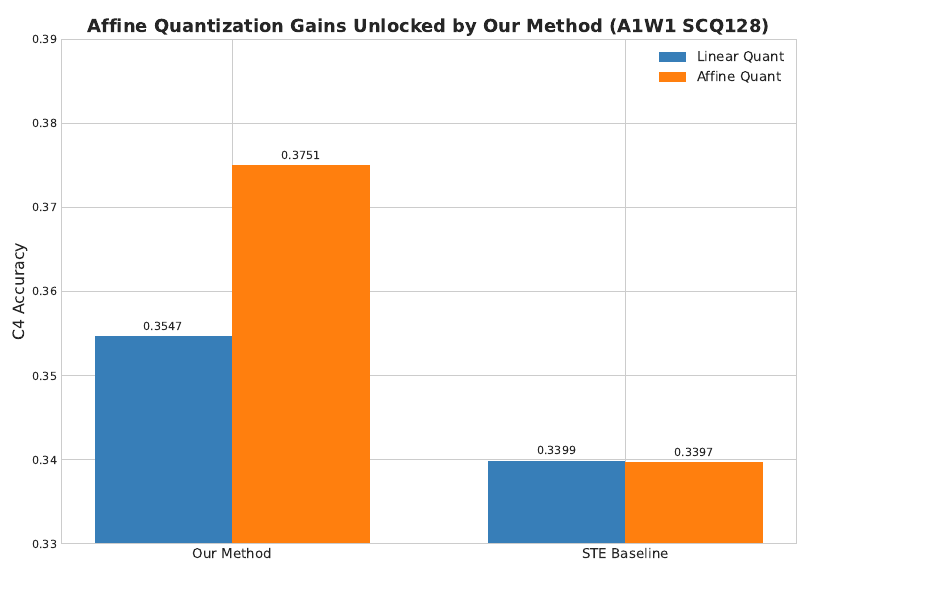
\includegraphics[width=\linewidth]{figs/fig1b_affine.png}\\[4pt]
\small Accuracy at A1W1, linear vs.\ affine quantization. Under STE affine gives no gain; with the paper's method it does.
\end{minipage}

\vfill
\noindent{\small\textit{Source:} Ye et al., ``Robust Training of Neural Networks at Arbitrary Precision and Sparsity,'' ICLR 2026, Fig.~1.}

\slide{The fix: ridge regression dequantization}

\slide{Why it works: the Jacobian sees $\delta$}

\slide{Role of $\lambda$}

\slide{Sparsity as quantization}

\slide{Theorem 1}

\slide{Results from the paper}

\slide{Toy implementation}

\paragraph{Model.} A small character-level GPT (decoder-only transformer): 4 blocks, 4 attention heads, embedding size 128, context of 64 characters, 0.82M parameters. Built following Karpathy's ``Let's build GPT: from scratch'' and nanoGPT, the same family as the paper's nanoGPT Shakespeare experiment.

\paragraph{Data.} Tiny Shakespeare: 1.1M characters, 65-character vocabulary, first 90\% for training, last 10\% for validation. Task: predict the next character.

\paragraph{Quantization.} All linear layers inside the transformer blocks, weights and input activations, $k$ bits (A$k$W$k$), affine, one $s_f$, $b_f$ per row. Embeddings and the output layer stay full precision.

\paragraph{Runs.} Same seed, AdamW (lr $10^{-3}$), batch 64, 3000 steps; only the dequantization step differs. Float (no quantization, baseline); STE, $\hat x=s_f\,q+b_f\mathbf 1$; ridge, $g(q)=s_g\,q+b_g\mathbf 1$ with $\lambda=0.01$. STE and ridge at $k=1,2,4$.

\vfill
\noindent{\small\textit{References:} A.~Karpathy, ``Let's build GPT: from scratch, in code, spelled out'' (2023) and nanoGPT, \texttt{github.com/karpathy/nanoGPT}; Tiny Shakespeare from \texttt{github.com/karpathy/char-rnn}.}

\slide{Toy implementation: results}

\noindent
\begin{minipage}[t]{0.49\textwidth}\centering
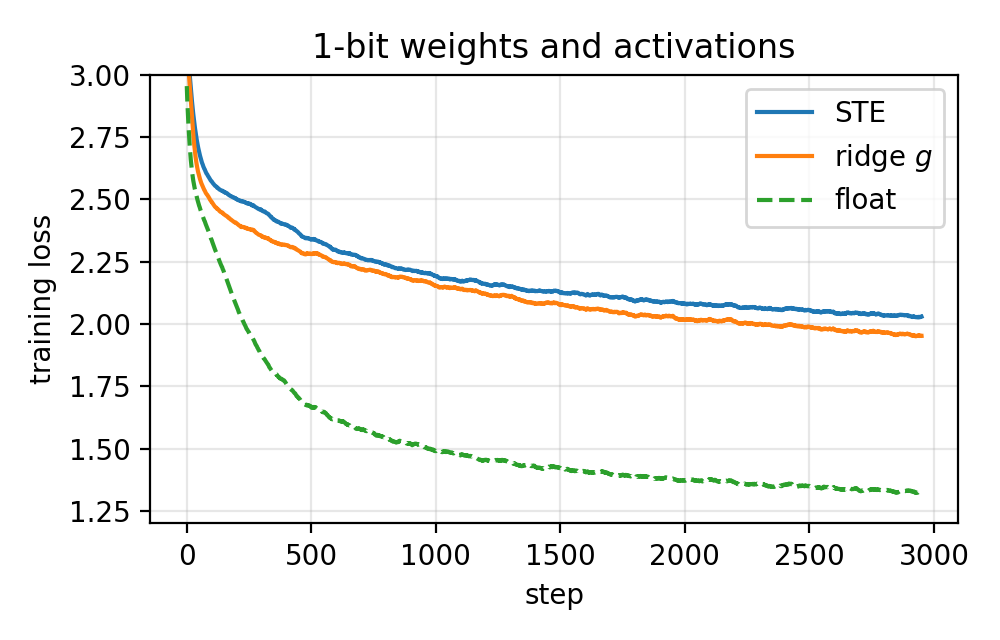
\includegraphics[width=0.85\linewidth]{implementation/plots/loss_k1.png}\\[4pt]
\small Training loss at A1W1 (smoothed over 50 steps).
\end{minipage}\hfill
\begin{minipage}[t]{0.49\textwidth}\centering
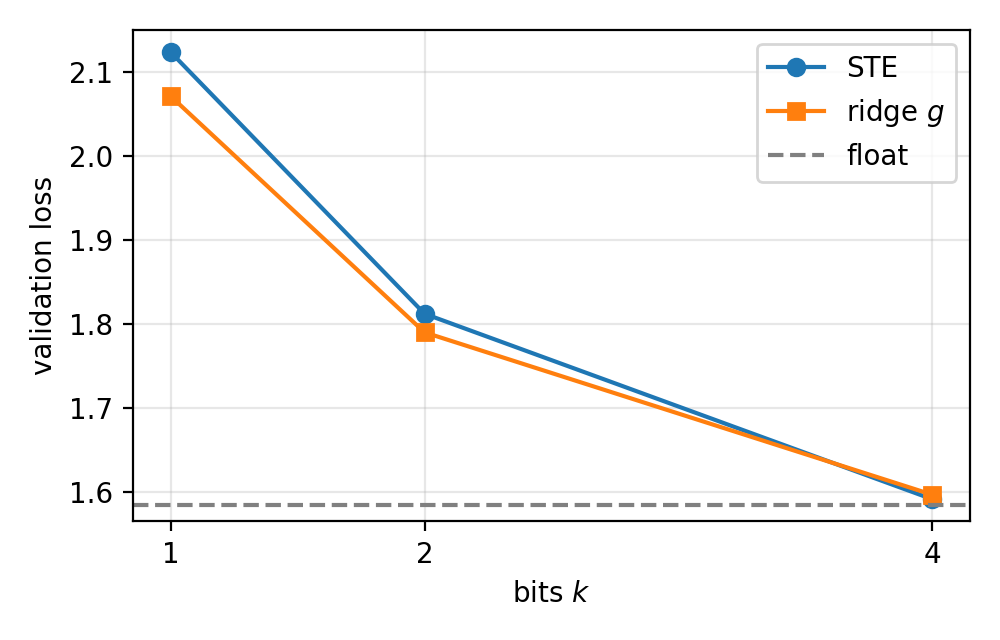
\includegraphics[width=0.85\linewidth]{implementation/plots/val_vs_bits.png}\\[4pt]
\small Final validation loss after 3000 steps.
\end{minipage}

\vspace{8pt}\noindent
\textbf{Gradient check} (1 bit, block of 64). Two inputs with the same $q$, rounding errors $\delta$ differing by up to 0.106, same upstream gradient:
\begin{center}\small
\begin{tabular}{lcc}
 & change in $\delta$ & change in gradient reaching $x$\\\hline
STE & 0.106 & 0.0000\\
ridge & 0.106 & 0.0144
\end{tabular}
\end{center}

\noindent\textbf{Size.} Float32 model 3.19 MB; at 1 bit 250 KB (12.7$\times$ smaller).

\slide{Limitations and how to improve}

\slide{Takeaway}

\end{document}
